Um die Funktionsweise beider Methoden zu belegen wurden diese sowohl auf ihre Robsutheit als auch auf ihre Performance getestet. Im folgenden Kapitel wird zunächst das zum Testen verwendete Setup beschrieben. Anschliessend erfolgt die Auswertung der erlangten Testergebnisse. Zuletzt werden weitere Tests durchgeführt welche das System kritischen Situationen testen soll.

% ---------------------- section -----------------------
\section{Testsetup}
\label{sec:test_setup}

Bei der Durchführung der Tests befinden sich die Kameras statisch im Raum. Die zu erkennenden Hindernisse werden innerhalb und ausserhalb der zu erkennenden Reichweite platziert, wobei die Ausrichtung der Hindernisse teils zufällig, teils bewusst an kritischen Positionen erfolgt um ein reales Anwendungsszenarien passend zu simulieren. Ein aufgenommenes Testset besteht dabei aus beiden Bildern der Kamera, der normalisierten Disparitätenkarte sowie eine komplette Punktwolke dieser um etwaige Fehler der Algorithmen leichter erkennen zu können, sowie den einzelnen Punktwolken der Hinderniserkennung. Weiterhin werden diverse Parameter gespeichert, wie die Anzahl der erkannten Hinderniselemente sowie deren Disparitäten.\\

\noindent
Der zu erkennende Bereich wurde auf $0,2$ bis $1,5$ Meter definiert. Dies entspricht einem Szenario in welchem das System auch aufgrund der hohen Framerate der Erkennung angewendet werden kann. Eine Erweiterung dessen auf beispielsweise $2.0$ Meter wurde nicht durchgeführt, da der Algorithmus auch bei großen Entfernungen robuste Werte in der Distanzberechnung liefert \cite{hilleralhallak}. Das nach der Anwendung der ROI auf die Disparitätenkarte erhaltene Sichtfeld (siehe \ref{sec:preprocessing}) beträgt $50^{\circ}$ auf horizontaler Achse und $38^{\circ}$ vertikal. Dies ist in Abbildung \ref{fig:field_of_view} visualisiert.
	
	\begin{figure}
		\centering
		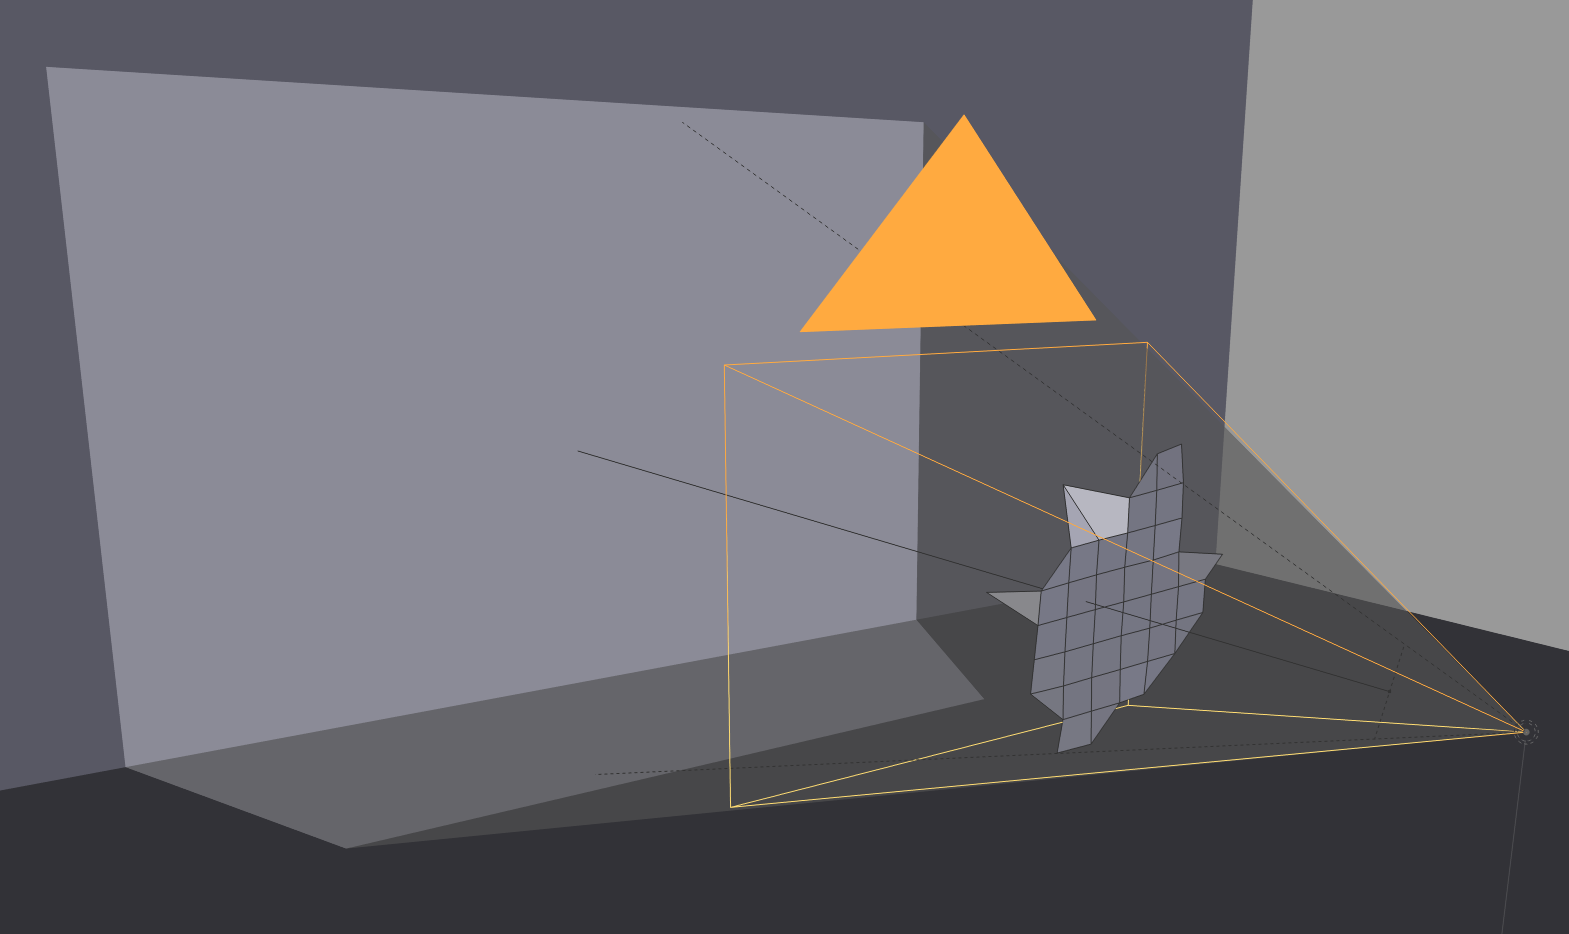
\includegraphics[width=8cm]{img/viewport}
		\caption{Im Bild ist das nach der Rektifizierung sowie Beschneidung der ROI erhaltene Sichtfeld visualisiert. Das Mesh innerhalb des Kamera Frustums repräsentiert die gerenderte Pointcloud eines Hindernisses}
		\label{fig:field_of_view}
	\end{figure}

\noindent
Ein aufgenommenes Testset besteht aus jeweils 12 Testbildern. Für jede Methode wurden drei verschiedene Hindernisgrößen getestet, groß, mittel und kleine Hindernisse. Anhand dieser wird ausgewertet welche minimale, maximale sowie mittlere Disparität, und daraus resultierende Distanz erkannt wird.\\

\noindent
% TODO checken welche tests final noch in der arbeit enthalten sind
Weitere Tests beinhalten die Erkennung kleiner Hindernisse unter Veränderung der \emph{SGBM} Parameter. Dabei wird unter anderem untersucht ob beispielsweise eine verringerte Blockgröße Einfluss auf die Erkennung kleiner Bereiche nimmt. Da die Samplepoint Detection den Radius als modifizierbaren Parameter mit sich bringt, wird auch dahingehend untersucht inwiefern die Wahl eines anderen Radius die Ergebnisse der Erkennung beeinflusst. Des Weiteren wird die Zeit für die Hinderniserkennung eines Frames untersucht um eine durchschnittliche Zeit für die Erkennung sowie die daraus resultierende Framerate zu ermitteln. Dies geschieht durch die Erkennung eines Hindernisses, welches sich über das gesamte Bild ausbreitet, sowie für nur ein Teilelement jeder Erkennungsmethode (Subimage, Samplepoint). Zudem wird geprüft inwiefern die Algorithmen mit Limitierungen des \emph{SGBM} umgehen können. Dazu zählen die Erkennung bei spiegelnden, reflektierenden und durchsichtigen Flächen, sowie die Erkennung schwach texturierter Hindernisse. Der letzte Test umfasst die Steigerung der Performance hinsichtlich der Veränderung der ursprünglichen Bildgröße bei der Erstellung der Disparitätenkarte.\\

% TODO bilder pre scaling 
% TODO weitere tests: spiegelnde flächen bilder aufnehmen und nach winkel evaluieren ob ein Hindernis erkannt wird
% TODO samplpoint radius veränderung
% TODO 

% TODO BILDER AUFNEHMEN

% ---------------------- section -----------------------
\section{Evaluierung Subimage Detection}
\label{sec:evaluierung_subimage}

 % TODO FIX COVERED AREAS AS RESULT OF BIGGER FONT SIZE
Hinsichtlich der Robustheit werden beide Algorithmen nach demselben Schema untersucht. Der in Abschnitt \ref{sec:test_setup} beschriebene Testablauf erwähnt 3 verschiedene Hindernisgrößen. Tabelle \ref{tbl:obstacle_sizes} zeigt sowohl die Maße der Hindernisse als auch deren Fläche in $cm/cm^2$ auf. Weiterhin werden die verwendeten Hindernisse in Abbildung REF dargestellt.
% TODO hindernisform: bilder warum benutzt
\begin{table}[h]
\centering
\begin{tabular}{|l|c|c|c|c|}
\hline
Hindernis   & Radius & Länge & Breite & Fläche \\
\hline
Groß   		&   -    & 53.5  & 43.0   & 2300.5 \\
\hline
Mittel 		& 	-    & 16.0  & 14.5   & 232.0\\
\hline
Klein		&  2.5	 &   -   &   -    & 19.6 \\
\hline	
\end{tabular}
\caption{Maße der verschiedenen genutzten Hindernisse}
\label{tbl:obstacle_sizes}
\end{table}


\noindent
Während der Tests wurde für jedes aufgenommene Einzelbild die reale Distanz gemessen. Der dabei verwendete Referenzpunkt befand sich in der Mitte des zu erkennenden Hindernisses, da diese nicht zwangsläufig orthogonal zur Bildebene platziert wurden. Somit entspricht die gemessene Distanz der mittleren Distanz welche sich aus allen gefundenen Bereichen eines Bildes zusammensetzt. Während der Aufnahme sind die jeweiligen Einzelbilder der linken und rechten Kamera sowie die berechnete Disparitätenkarte sichtbar. Zudem ist ein weiterer Anzeigemodus verfügbar welcher die gefundenen Hindernisse innerhalb der Tiefenkarte markiert (siehe Abbildung \ref{fig:test_viewing}). Weiterhin kann jede erstellte Hindernis-Pointcloud im Nachhinein gerendert werden um einen überblick über die Ergebnisse des Algorithmus zu erhalten.\\

\begin{figure}[h]
	\centering
	\begin{tabular}{c c}
	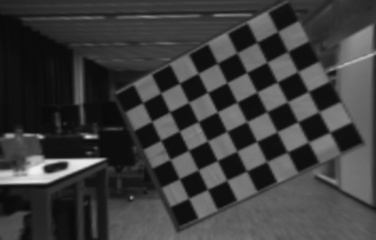
\includegraphics[width=5.0cm]{img/evaluation/test_set/_test_3_left}&
	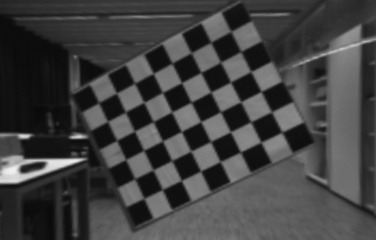
\includegraphics[width=5.0cm]{img/evaluation/test_set/_test_3_right}\\
	(a) linkes Kamerabild & (b) rechtes Kamerabild\\
	
\includegraphics[width=5.0cm]{img/evaluation/test_set/_test_3_disparity}&
    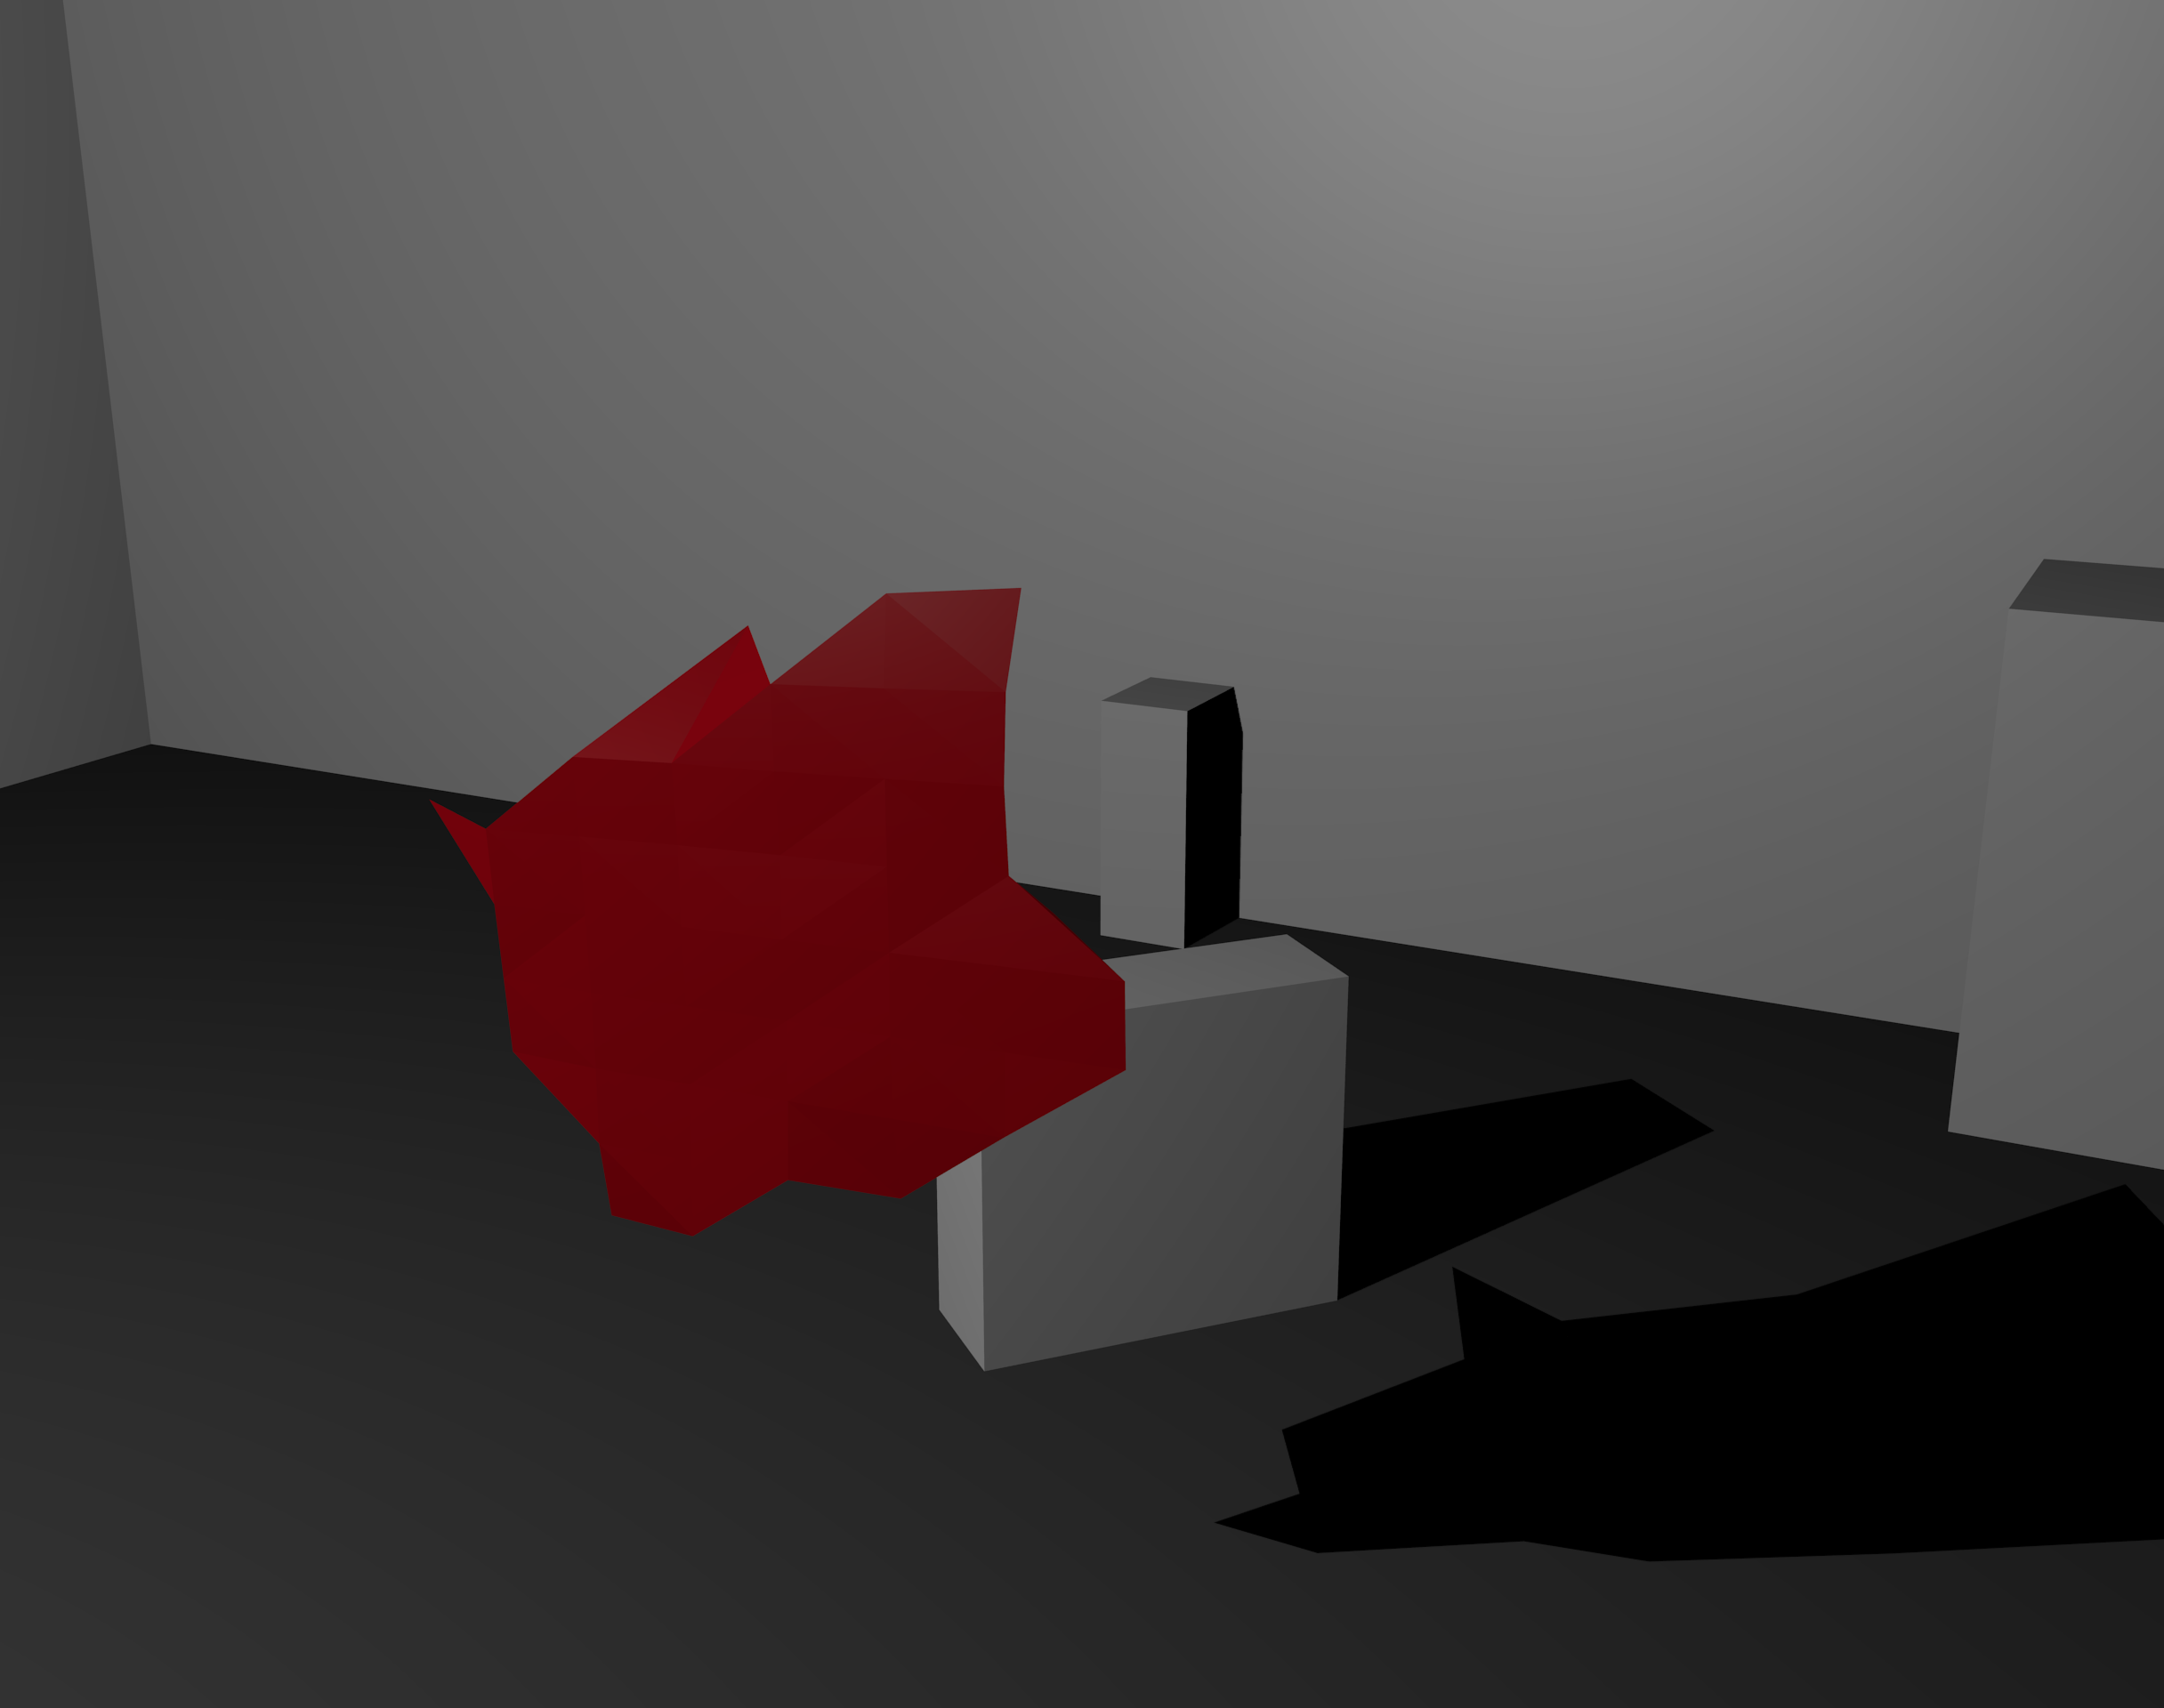
\includegraphics[width=5.0cm]{img/evaluation/test_set/rendered_obstacle}\\
	(c) Anzeigemodus Hindernis & (d) Hindernis Pointcloud als Mesh
	\end{tabular}
	\caption{Abbildungen (a) - (c) zeigen die sichtbaren Bilder während der Testaufnahme. (c) zeigt eine als Mesh gerenderte Pointcloud}
	\label{fig:test_viewing}
\end{figure}


\noindent
\textbf{Großes Hindernis:}\\ 
\noindent
Im ersten Test wurde das große Hindernis gewählt, dabei wurde mithilfe der dargestellten Hindernisse auf der Disparitätenkarte überprüft ob sich die erkannten Hindernisse innerhalb des Gefahrenbereichs befinden. Um auch kritische Bereiche zu testen wurde das Hindernis zudem zu Teilen außerhalb dieser platziert. Aus den 12 aufgenommenen Bildern des Testsets ergaben sich die in Abbildung \ref{fig:eval_big} (a) sichtbaren Ergebnisse.\\

\begin{figure}[h]
	\centering
	\begin{tabular}{cc}
	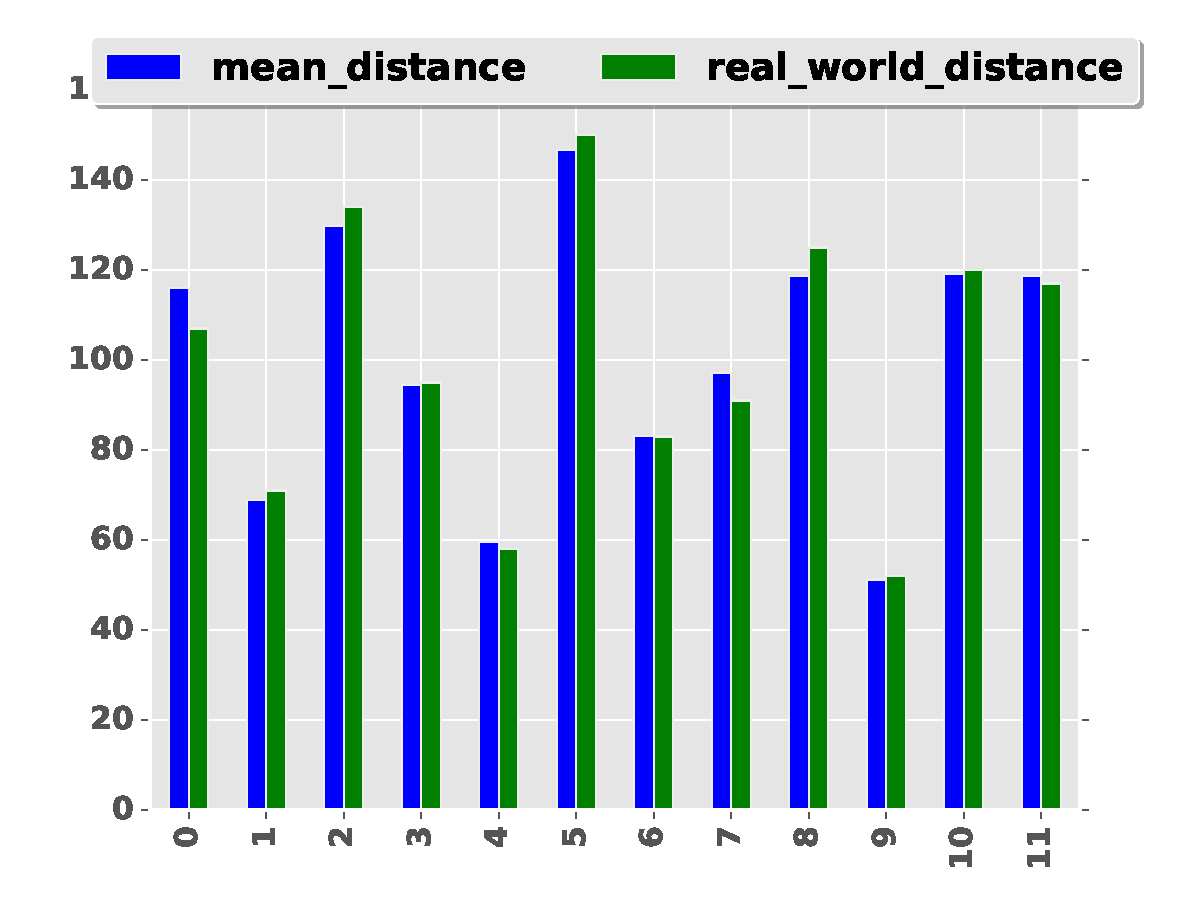
\includegraphics[width=7cm]{img/evaluation/diagrams/sub_big_bar}&
	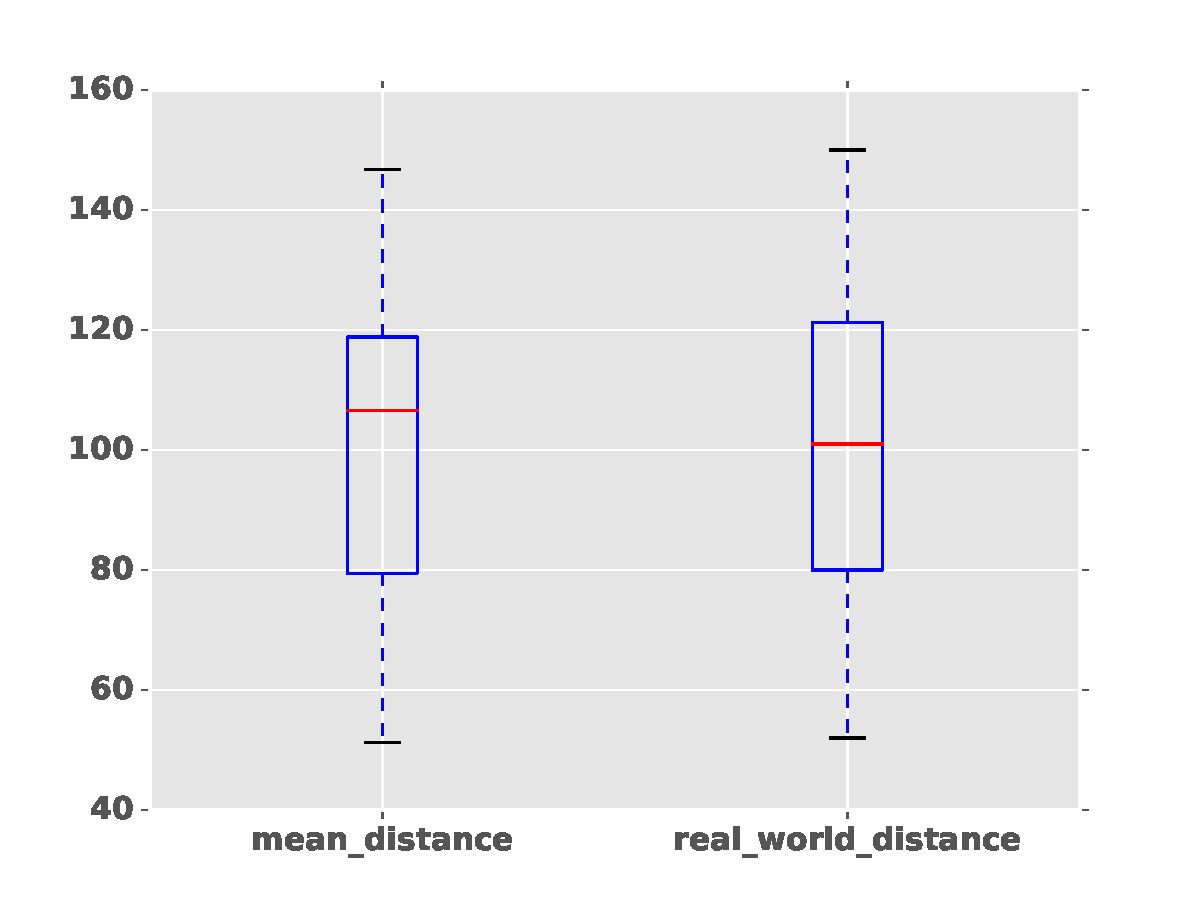
\includegraphics[width=7cm]{img/evaluation/diagrams/sub_big_box}\\
	 (a) & (b)
	\end{tabular}
	\caption{}
    \label{fig:eval_big}
\end{figure}

\noindent
Wie aus diesen zu erkennen wurde in nahezu allen Frames das Hindernis richtig erkannt. Die berechneten Distanzen stimmen mit den real gemessenen überein. Minimale Abweichungen können in diesem Fall als Messungenauigkeit ignoriert werden, da der Mittelpunkt zwischen der minimalen und maximalen Objektdistanz kein statischer Punkt ist. Zwar wurden alle Hindernisse erkannt, jedoch nicht der gesamte Bereich den sie umfasst haben. Wie Abbildung \ref{fig:eval_big_fails} zeigt wurden der obere und untere Bereich des Hindernisses im 5. Frame nicht erkannt. Dies könnte einerseits aus der Rotation des Objektes resultieren, andererseits auch aus einer gewissen Biegung die das physische Objekt mit sich bringt.

\begin{figure}[h]
	\centering
	\begin{tabular}{cc}
	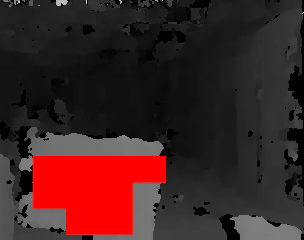
\includegraphics[width=5cm]{img/evaluation/_test_5_disparity}&
	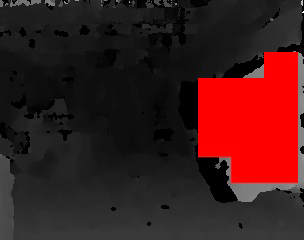
\includegraphics[width=5cm]{img/evaluation/_test_8_disparity}\\
	(a) Frame 5 &  (b) Frame 8
	\end{tabular}
	\caption{}
    \label{fig:eval_big_fails}
\end{figure}

\noindent
Auch im in Abbildung \ref{fig:eval_big} (b) abgebildeten Boxplot lässt sich erkennen, dass der Median beider gemessenen Distanzen, mit geringen Abweichungen, nahezu gleich ist. Auch die minimal und maximal Werte befinden sich, ebenfalls mit vernachlässigbaren Abweichungen auf derselben Gerade.\\

\noindent
\textbf{Mittleres Hindernis:}\\
\begin{figure}[h]
	\centering
	\begin{tabular}{cc}
	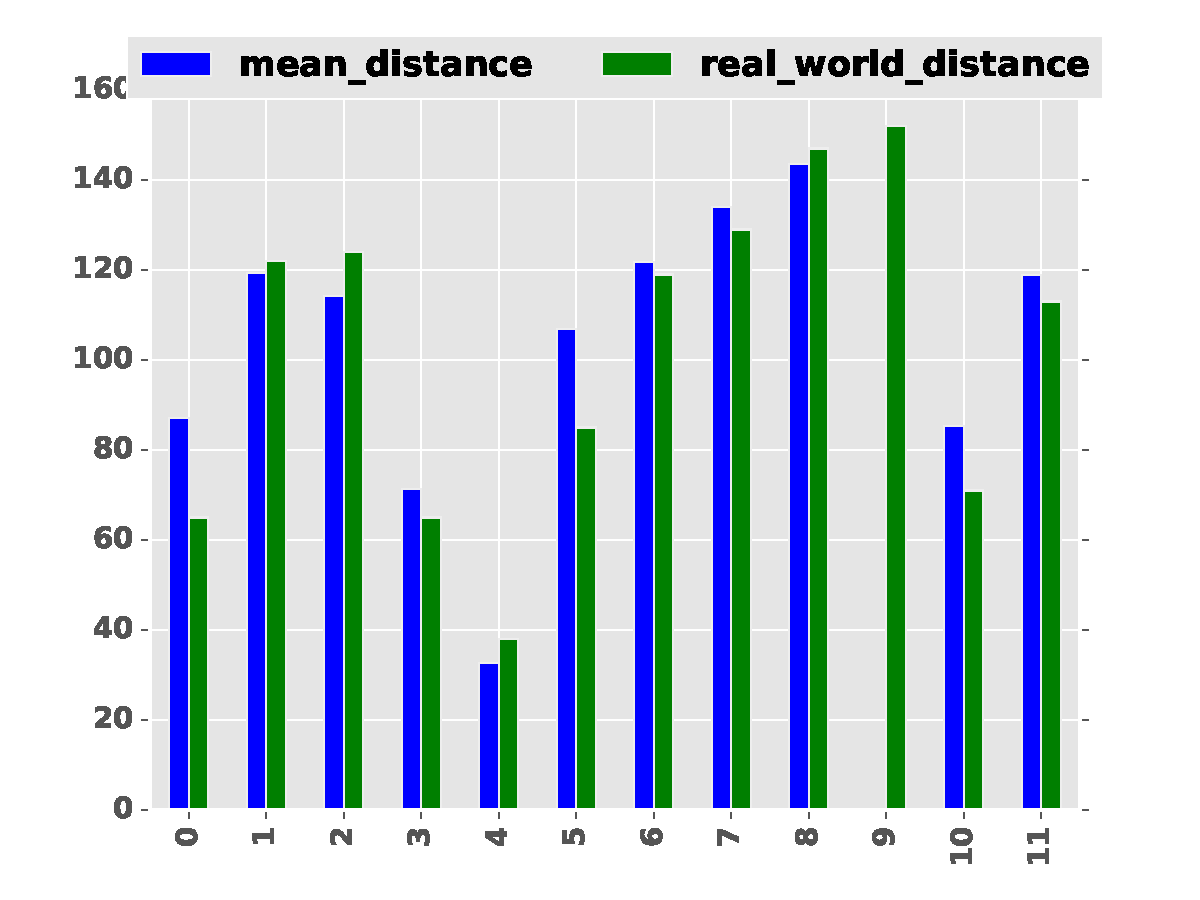
\includegraphics[width=7cm]{img/evaluation/diagrams/sub_medium_bar}&
	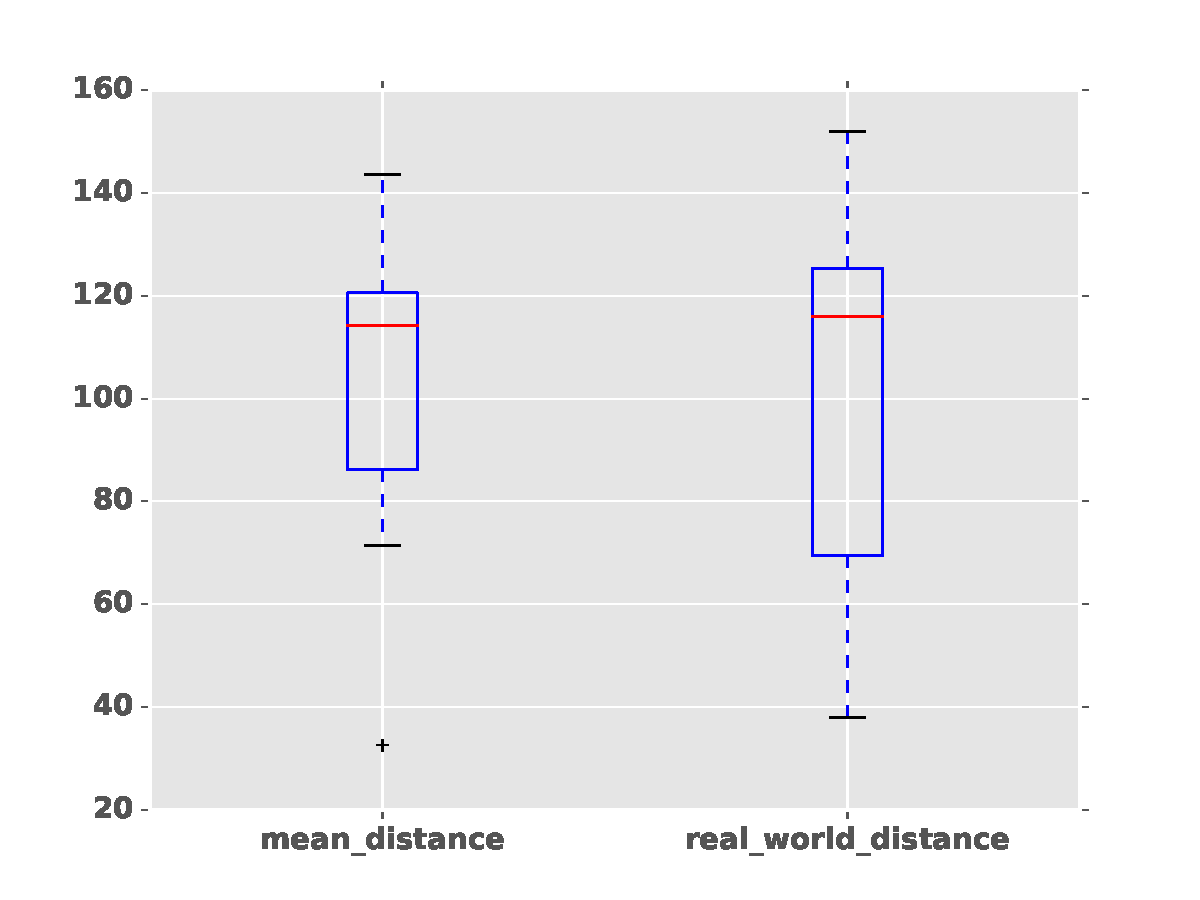
\includegraphics[width=7cm]{img/evaluation/diagrams/sub_medium_box}\\
	(a) &  (b)
	\end{tabular}
    \caption{}
    \label{fig:eval_medium}
\end{figure}

\noindent
Auch die Erkennung mittlerer Hindernisse durch den Algorithmus war in nahezu allen Fällen erfolgreich. Ein auffälliges Detail im Vergleich zu den Ergebnissen des großen Hindernisses ist die höhere Differenz aus berechneter und gemessener Distanz. Das getestete Objekt befand sich während der Tests an einem durchsichtigen Plexiglas Stab welcher teilweise auch als Hindernis erkannt wurde. Im Fall von Frame 0 umfasst das Objekt insgesamt 17 Subimages in denen es erkannt wurde. Als Resultat des Stabes wurden jedoch noch 2 weitere erkannt. Frame 1 weist zwar keine große Abweichung zwischen der berechneten und realen Distanz auf, jedoch wird das Objekt zu Teilen nicht erkannt. Bei einer Distanz von 120 Zentimetern ist eine Erkennung dieser Hindernisgröße in nur 2 Subimages ungewöhnlich. Dies könnte zum Teil aus der verwendeten Blockgröße resultieren.

\begin{figure}[h]
	\centering
	\begin{tabular}{cc}
	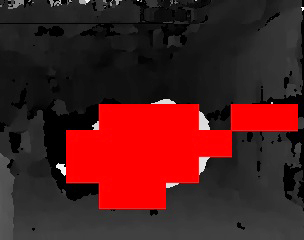
\includegraphics[width=5cm]{img/evaluation/medium_test_0_disparity}&
	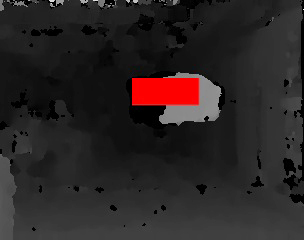
\includegraphics[width=5cm]{img/evaluation/medium_test_1_disparity}\\
	(a) Frame 0 &  (b) Frame 3
	\end{tabular}
	\caption{}
	\label{fig:eval_medium_fails}
\end{figure}

\noindent
Selbiges Resultat lässt sich in den Frames 2, 6 und 7 erkennen. In Frame 9 dagegen konnte kein Hindernis erkannt werde, da sich das Objekt an der Grenze der Gefahrenzone befunden hat und demnach die Abweichung der Disparität zu keiner Erkennung führen konnte. Eben diese Ergebnisse sind auch in Abbildung \ref{fig:eval_medium} (sb) sichtbar, das Maximum der realen Distanz resultiert dabei aus dem nicht erkannten Hindernis in Frame 9.\\

\noindent
\textbf{Kleines Hindernis:}\\
\begin{figure}[h]
	\centering
	\begin{tabular}{cc}
	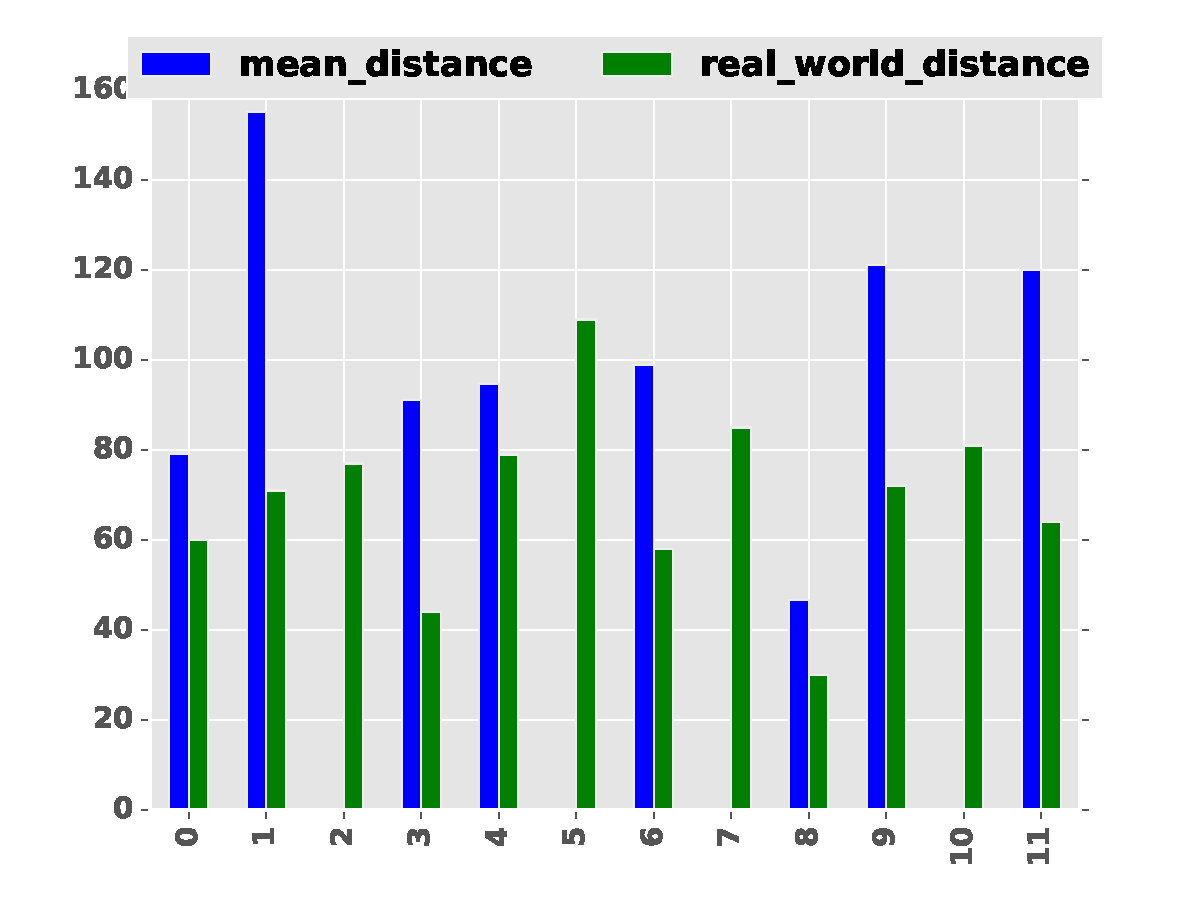
\includegraphics[width=7cm]{img/evaluation/diagrams/sub_tiny_bar}&
	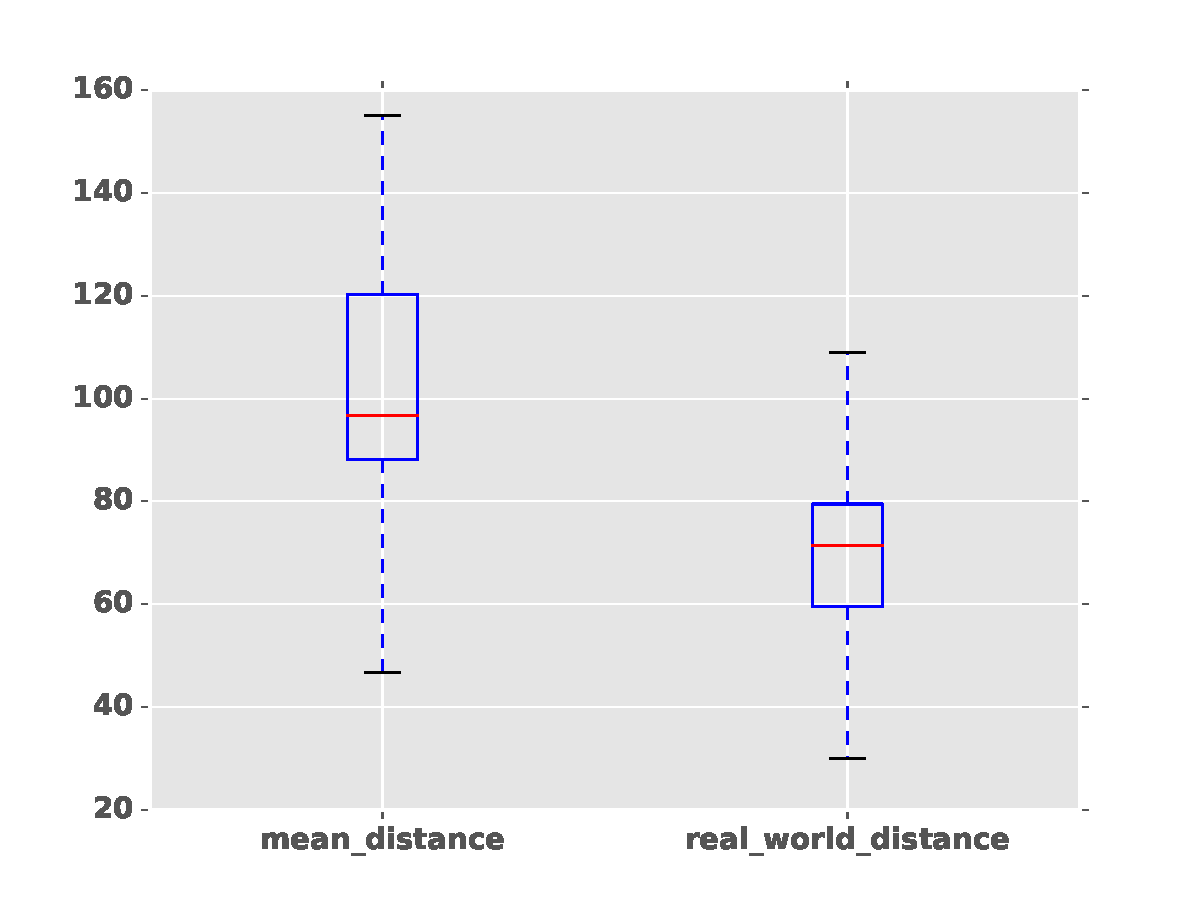
\includegraphics[width=7cm]{img/evaluation/diagrams/sub_tiny_box}\\
	(a)	& (b)
	\end{tabular}
    \caption{}
    \label{fig:eval_tiny}
\end{figure}

\noindent
Die Erkennung kleiner Hindernisse gestaltet sich aufgrund diverser Faktoren schwer. Ein limitierender Faktor ist die Fläche, ist ein einzeles Hindernis so klein, dass es während der Berechnung des Medians aufgrund der umliegenden Disparitäten untergeht, so kann auch kein Hindernis erkannt werden. Dies macht sich in vielen der getesteten Bildern bemerkbar. In den Frames 2, 5, 7 und 10 wurde das Hindernis nicht erkannt, da es sich entweder an einer Kreuzung verschiedener Subimages befand, oder die verwendete Blockgröße nicht ausreicht, dadurch wird der Median aller Teilmatrizen nicht signifikant beeinflusst. Auch der Stab wurde in den Frames 3, 6 sowie 8 als zusätzliches Hindernis erkannt. Dies ist ein Resultat der relativ geringen Distanz zu den Kameras. Die hohen Entfernungsdifferenzen resultieren in diesen Fällen wiederum aus der großen Entfernung der Hindernisse zum Hintergrund sowie dem auftretenden \enquote{Schatten} welcher durch die Baseline zu begründen ist. Auch der in Abbildung \ref{fig:eval_tiny} (b) dargestellte Boxplot zeigt, das signifikant größere Distanzen erkannt wurden als sie in den realen Messungen vorkommen.

% ---------------------- section -----------------------
\section{Evaluierung Samplepoint Detection}
\label{sec:evaluierung_samplepoint}

\noindent
Durch die wesentlich höhere Anzahl an betrachteten Bereichen innerhalb der Disparitätenkarte ist anzunehmen, dass die Erkennung kleiner Hindernisse eine höhere Erfolgswahrscheinlichkeit verspricht. Im Rahmen dieses Abschnittes wird die Samplepoint Detection getestet. Dies geschieht nach dem in \ref{sec:evaluierung_subimage} bereits beschriebenen Schema. Zur Initialisierung der Methode wurde der Radius der Samplepoints auf 2 Pixel gesetzt, was einer Gesamtanzahl von 25 Pixeln pro Samplepoint entspricht.\\

\noindent
\textbf{Großes Hindernis:}\\
Die Erkennung großer Objekte der Samplepoint Detection weist nahezu keine Fehler auf. Abbildung \ref{fig:sample_eval_big} zeigt das jede der 12 Ausrichtungen des Objektes erkannt wurden. Die dabei auftretenden Differenzen zwischen der berechneten sowie gemessenen Distanz sind auf Messungenauigkeiten zurückzuführen. Auch in Grenzbereichen nahe dem Rand des Gefahrenbereichs wurden die Hindernisse erkannt. 

\begin{figure}[h]
	\centering
	\begin{tabular}{cc}
	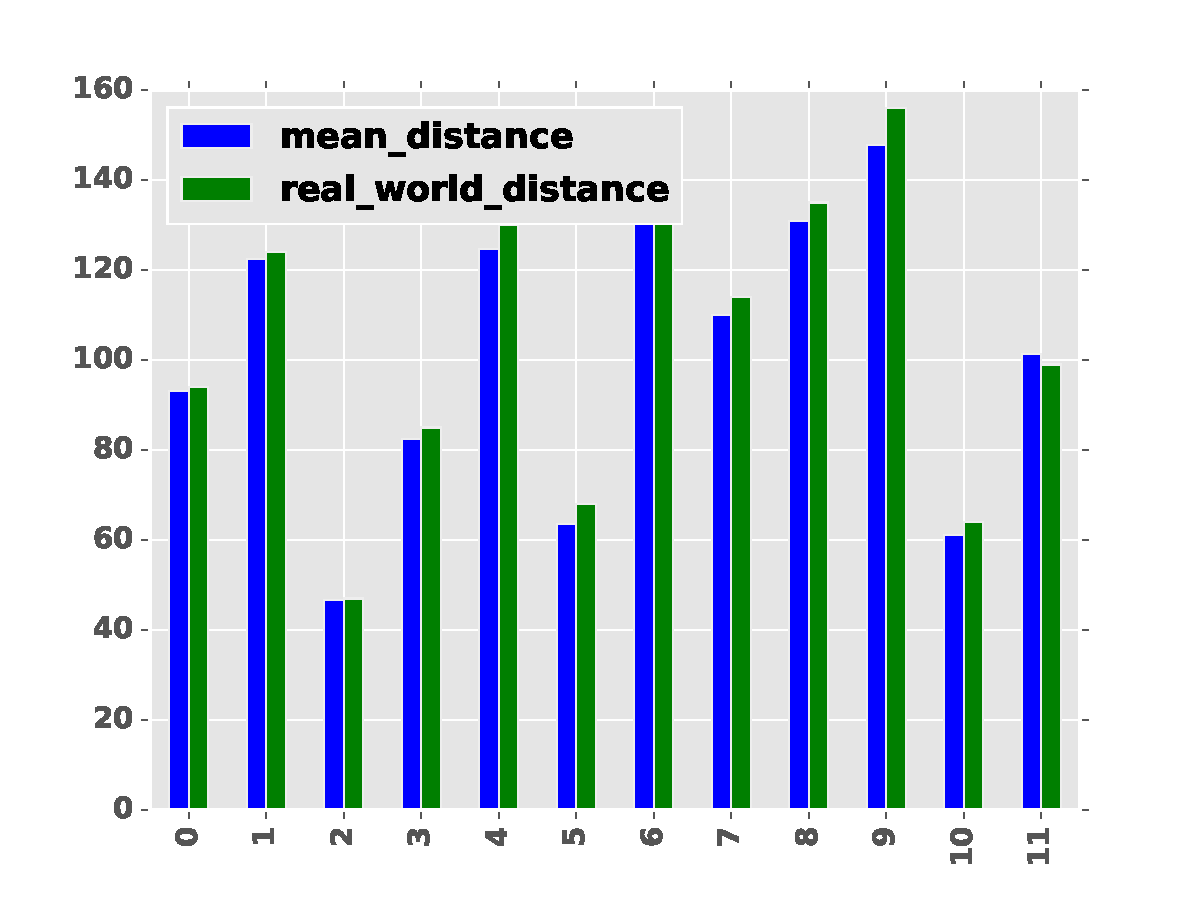
\includegraphics[width=7cm]{img/evaluation/diagrams/sample_big_bar}&
	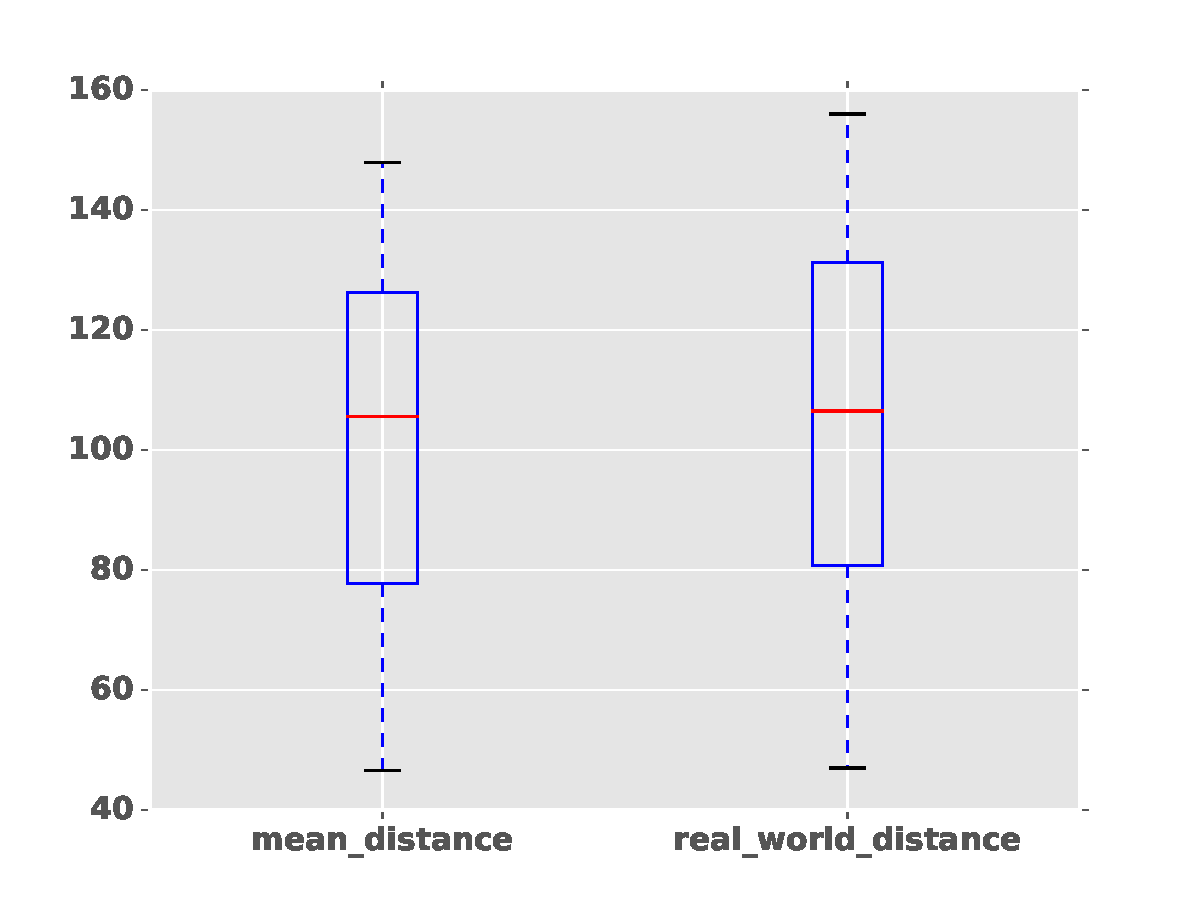
\includegraphics[width=7cm]{img/evaluation/diagrams/sample_big_box}\\
	 (a) & (b)
	\end{tabular}
	\caption{}
    \label{fig:sample_eval_big}
\end{figure}

\noindent
\textbf{Mittleres Hindernis:}\\

\begin{figure}[h]
	\centering
	\begin{tabular}{cc}
	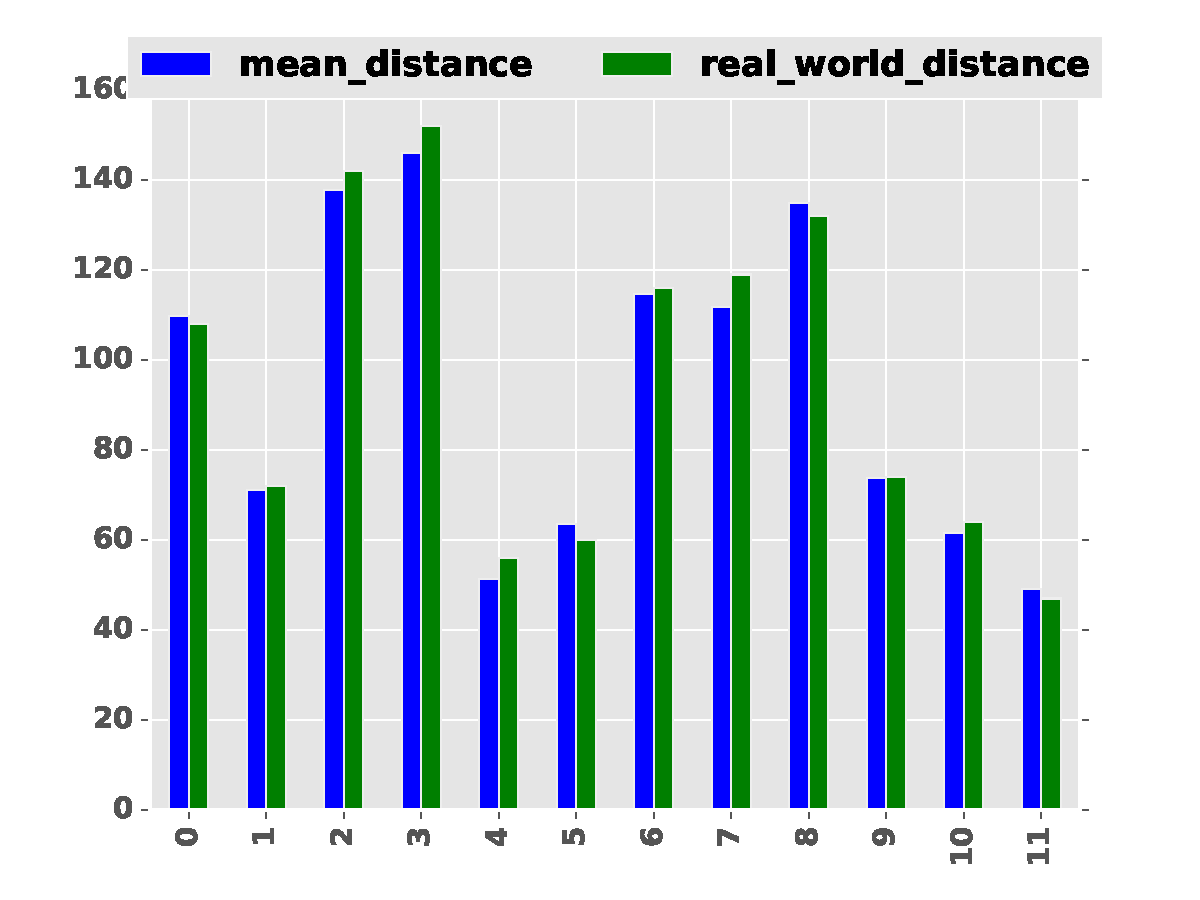
\includegraphics[width=7cm]{img/evaluation/diagrams/sample_medium_bar}&
	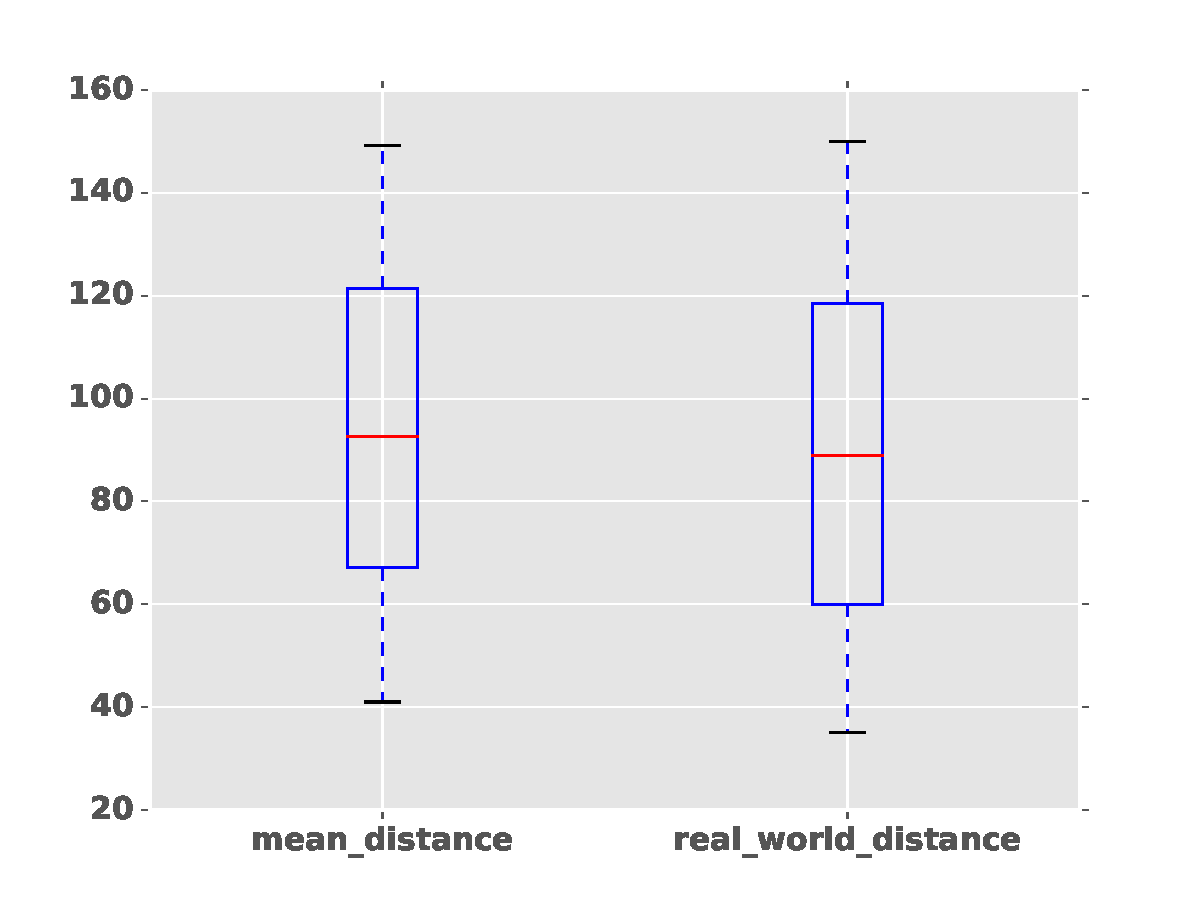
\includegraphics[width=7cm]{img/evaluation/diagrams/sample_medium_box}\\
	 (a) & (b)
	\end{tabular}
	\caption{}
    \label{fig:sample_eval_medium}
\end{figure}

\noindent
Auch die Erkennung mittlerer Hindernisse erfolgte in allen Frames ohne signifikante Probleme (siehe Abbildung \ref{fig:sample_eval_medium}). Bereiche in denen aufgrund fehlender Textur keine Korrespondenz zugeordnet werden konnte wurden aufgrund der hohen Dichte der Samplepoints trotzdem erkannt. Wie Abbildungen \ref{fig:sample_eval_medium_fails} (a) und (b) zeigen wurden nicht gematchte Bereiche auch nicht als Hindernis erkannt, die umliegenden texturierten Bereiche überwiegen jedoch und sorgen daher für eine robuste Detektion.

\begin{figure}[h]
	\centering
	\begin{tabular}{cc}
	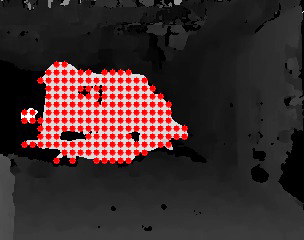
\includegraphics[width=5cm]{img/evaluation/sample_tiny_test_5_disparity}&
	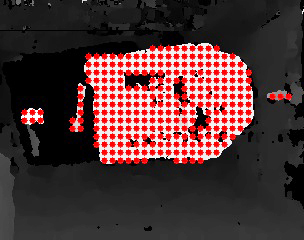
\includegraphics[width=5cm]{img/evaluation/sample_tiny_test_11_disparity}\\
	(a) Frame 5 &  (b) Frame 11
	\end{tabular}
	\caption{}
	\label{fig:sample_eval_medium_fails}
\end{figure}

\noindent
Die bereits beschriebene hohe Dichte der Samplepoints und deren geringe Größe hilft auch hier wieder den Stab als Hindernis zu erkennen (siehe Abbildung \ref{fig:sample_eval_medium_fails} (b))\\


\noindent
\textbf{Kleines Hindernis:}\\
Die anfangs anfänglich aufgestellte These, dass sich die Verteilung sowie Größe der Samplepoints positiv auf die Erkennung diverser Hindernisse auswirkt wird mit den Ergebnissen des kleinen Hindernisses bestätigt. Diagramm \ref{fig:sample_eval_tiny} (a) belegt diese Aussage. Es wurden alle 12 Hindernisse ohne signifikante Differenz in den Distanzen erkannt. Trotz dessen ist die Detektion dieser bei Entfernungen von mehr als 60 Zentimetern stark von der Orientierung des Objektes, dem Hintergrund sowie den verwendeten Parametern zur Berechnung der Disparitätenkarte abhängig. Da die geringe Auflösung der Kameras keine detaillierte Aufnahme der Textur des Hindernisses zulässt ist es möglich das das Objekt aufgrund der Blockgröße des \emph{SGBM} mit dem Hintergrund zusammen gematcht wird. 

\begin{figure}[h]
	\centering
	\begin{tabular}{cc}
	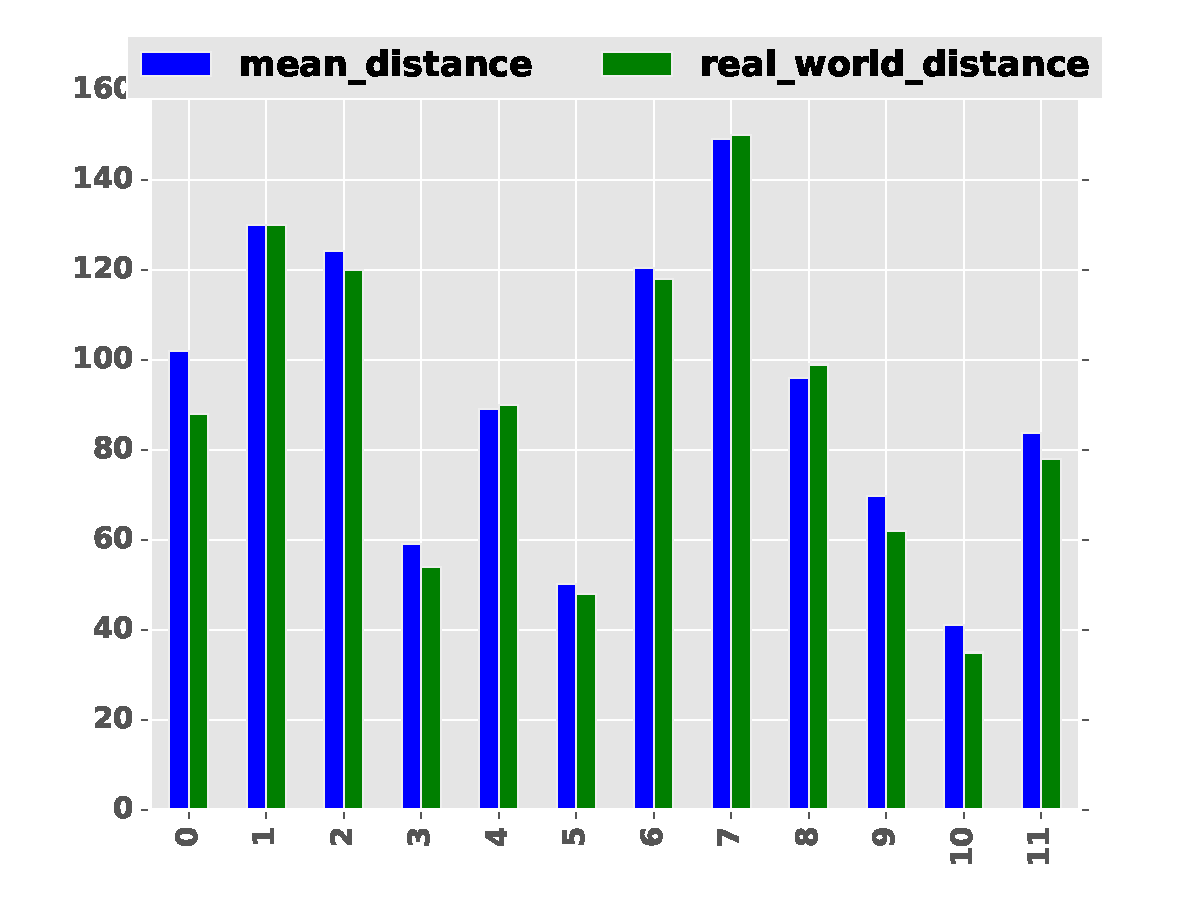
\includegraphics[width=7cm]{img/evaluation/diagrams/sample_tiny_bar}&
	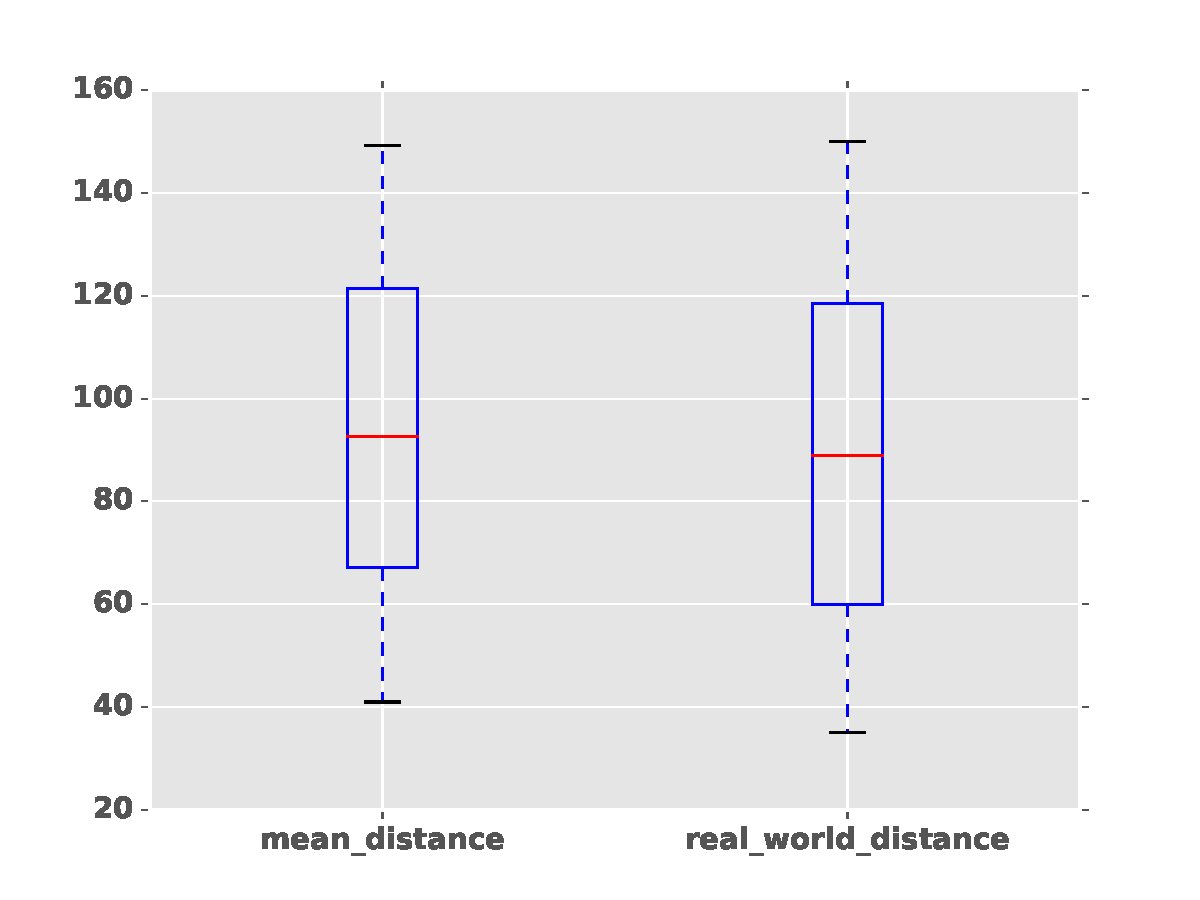
\includegraphics[width=7cm]{img/evaluation/diagrams/sample_tiny_box}\\
	 (a) & (b)
	\end{tabular}
	\caption{}
    \label{fig:sample_eval_tiny}
\end{figure}

\noindent
Weiterhin ist auch die statistische Auswertung der Distanzen in Boxplot \ref{fig:sample_eval_tiny} (b) ein Zeichen für die robuste Erkennung kleiner Hindernisse. Lediglich das untere Quartil der berechneten Entfernungen weicht um ca. 6 Zentimeter von den realen Werten ab.

% ---------------------- section -----------------------
\section{Weitere Versuche}
\label{sec:further_tests}

Hinsichtlich der verschiedenen möglichen Faktoren welche eine erfolgreiche Erkennung beeinflussen können wurden im Rahmen der Evaluation beider Algorithmen weitere Tests durchgeführt. Jene umfassen die Erkennung kleiner Hindernisse unter Veränderung der Größe des Matching-Blocks. Weiterhin wird die Erkennung kritischer Umgebungen (durchsichtige, reflektierende und homogener Flächen) getestet. Anschließend erfolgt ein weiter Versuch welcher auf die Veränderung des Samplepoint Radius und die damit verbundenen Änderungen in der Erkennung abzielt. Das während des Tests genutzte Setup wurde während der Aufnahme nicht verändert. Auch das Objekt befand sich für jede Blockgröße an der jeweiligen Distanz. Zur Durchführung der Tests wurde das in Abschnitt \ref{sec:evaluierung_subimage} und\ref{sec:evaluierung_samplepoint} genutzte kleine Hindernis verwendet.

\noindent
\subsection{Veränderung der \emph{SGBM} Block Größe}
\label{subsec:block_size_change}

\textbf{Subimage Detecion:}\\
\noindent
Um die Auswirkungen der Blockgröße auf die Distanzberechnung zu testen wurden verschiedene Kantenlängen des Blocks getestet. Für jede Größe wurde die Hinderniserkennung aus je 3 Distanzen ausgeführt. Im Folgenden werden zunächst die Daten dargelegt und im Anschluss daran analysiert. Eine Diskussion der erhaltenen Ergebnisse findet in Abschnitt \ref{sec:gegenueberstellung} statt.\\
	
\begin{table}[h]
\centering
\begin{tabular}{|l||c|c|}
\hline
Blockgröße & berechnete Distanz & real gemessene Distanz \\
\hline\hline
7          & 120.6          		& 50                     \\
           &  -                 & 100                    \\
           &  -                 & 150                    \\
\hline
9          & 105.8          		& 50                     \\
           &  -                 & 100                    \\
           &  -                 & 150                    \\
\hline
11         & 98.9           		& 50                     \\
           &  -                 & 100                    \\
           &  -                 & 150                    \\
\hline
13         & 85.2          		& 50                     \\
           &  -                 & 100                    \\
           &  -                 & 150                    \\
\hline
15         & 112.1		        & 50                     \\
           &  -                 & 100                    \\
           &  -                 & 150                    \\
\hline
21         & 108.6         		& 50                     \\
           &  -                 & 100                    \\
           &  -                 & 150                    \\
\hline
\end{tabular}
\caption{Ausgewertete Daten des Subimage Sets}
\label{tbl:distance_subimage}
\end{table}	

\noindent
Wie aus Abbildung \ref{tbl:distance_subimage} ersichtlich wird hat eine Änderung der Blockgröße keine Auswirkungen auf die Erkennung des Objektes. Die berechneten Entfernungen werden erheblich von den Pixeln des Hintergrundes beeinflusst, was in den verzerrten berechneten Distanzen resultiert. Dabei auftretende Differenzen zwischen den real gemessenen Entfernungen sowie den berechneten resultieren aus Interferenzen während der Neuberechnung der Disparitätenkarte in jedem Frame.\\

\noindent
\textbf{Samplepoint Detection:}\\

\begin{table}[h]
\centering
\begin{tabular}{|l||c|c|}
\hline
Blockgröße & berechnete Distanz & real gemessene Distanz \\
\hline\hline
7          & 63.8               & 50                     \\
           & 102.2              & 100                    \\
           & 149.1              & 150                    \\
\hline
9          & 57.3               & 50                     \\
           & 107.9              & 100                    \\
           & 153.6              & 150                    \\
\hline
11         & 68.0               & 50                     \\
           & 107.1              & 100                    \\
           & 149.1              & 150                    \\
\hline
13         & 51.4               & 50                     \\
           & 101.4              & 100                    \\
           & 151.1              & 150                    \\
\hline
15         & 57.3               & 50                     \\
           & 105.3              & 100                    \\
           & 149.1              & 150                    \\
\hline
21         & 56.0               & 50                     \\
           & 101.5              & 100                    \\
           & 147.3              & 150                    \\
\hline
\end{tabular}
\caption{Ausgewertete Daten des Subimage Sets }
\label{tbl:distance_samplepoint}
\end{table}

\noindent
Die Änderung der Blockgröße hat auch bei der Samplepoint Detection keinen signifikanten Einfluss auf die Erkennung oder Berechnung der Hindernisdistanz. Jedoch ist die Differenz der Entfernungen bei 13 Pixeln Blockgröße am geringsten. Während der einzelnen Versuche wurde der Befestigungsstab des Hindernisses ebenfalls erkannt (siehe Abbildung \ref{fig:distance_sample_images}).

\begin{figure}[h]
	\centering
	\begin{tabular}{ccc}
	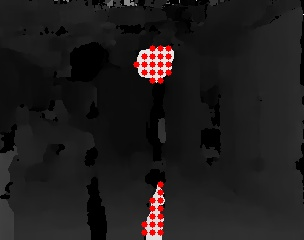
\includegraphics[width=4cm]{img/evaluation/distance_sample/_test_0_disparity}&
	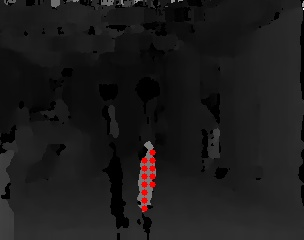
\includegraphics[width=4cm]{img/evaluation/distance_sample/_test_1_disparity}&
	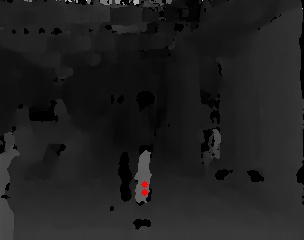
\includegraphics[width=4cm]{img/evaluation/distance_sample/_test_2_disparity}
	\end{tabular}
	\caption{Testset unter Verwendung einer Blockgröße von 13 Pixeln in verschiedenen Distanzen (50 cm bis 150 cm v.l.n.r.)}
	\label{fig:distance_sample_images}
\end{figure}

\noindent
Dabei lässt sich in allen Bildern welche im Abstand von 100 Zentimetern aufgenommen erkennen, dass das eigentliche Hindernis nicht mehr gefunden wurde, sondern die Befestigung dessen das erkannte Hindernis repräsentiert. Ein Grund für diese \enquote{falsch}-Erkennung könnte auch hier die Verwendung des Mittelwertes, sowie der nicht beachtete Raum zwischen den einzelnen Samplepoints sein. Bei einem Radius von 2 Pixeln beträgt dieser ebenfalls 2 Pixel. Eine Verzerrung der Werte durch den Hintergrund ist in diesem Fall unwahrscheinlich, die Verbindung der Distanz sowie der geringen Aufnahmeauflösung der Kameras führt eher dazu, dass das Hindernis vor dem Hintergrund als Teil dessen wirkt. Die plausibelste Fehlerquelle ist daher am wahrscheinlichsten die zugrunde liegende Disparitätenkarte.

% ---------------------- section -----------------------
\section{Diskussion}
\label{sec:evaluation_Diskussion}
% TODO allgemein mehr schreiben vielleicht

Die in den Abschnitten \ref{sec:evaluierung_subimage} und \ref{sec:evaluierung_samplepoint} erlangten Ergebnisse belegen die generelle Funktionsweise beider Algorithmen. Die Grundidee der Methoden gleicht sich in einigen Punkten, ebenso die Resultate. Beide Algorithmen liefern robuste Ergebnisse unter der Voraussetzung einer gewissen Hindernisgröße, wobei das kleine Objekt die größte Anforderung an diese stellt. Die Detektion des großen sowie mittleren Hindernisses ergab in allen Versuchen die Ergebnisse mit den niedrigsten Differenzen zwischen berechneten und gemessenen Entfernungen.\\

\noindent
Das Konzept der Subimage Detection ist in Bezug auf große und mittlere Hindernisse als robust einzustufen, jedoch ist die Berechnung des Medians der Matrizen auch der größte Konflikt. Weist der Hintergrund eines Objektes sehr geringe Disparitäten auf, so besteht die Möglichkeit das der Hintergrund den Mittelwert eines einzelnen Subimages insofern beeinflusst, dass das Hindernis (innerhalb dieser Submatrix) nicht mehr erkannt werden kann. Dies ließ sich bei nahezu allen Versuchen und Hindernisgrößen beobachten. Im Fall der großen und mittleren Hindernisse stellt dies keinen Konflikt dar, da die Fläche der Hindernisse trotzdem für eine Erkennung ausreicht. Ungeachtet dessen stellt gerade dieser Konflikt ein Problem in der Erkennung einzelner kleiner Hindernisse dar.\\

\noindent
Die Erkennung von Hindernissen mit Hilfe der Samplepoints ist ebenfalls eine robuste Methode. Dabei reicht die Anzahl der umfassenden Pixel eines jeden aus um selbst kleine Hindernisse zu erkennen. Der nicht beachtete Bereich zwischen den Samplepoints kann entweder 6, 4, 2 oder keinen Pixel betragen, in Abhängigkeit des verwendeten Radius. Dies reicht jedoch nicht immer um das eigentliche Hindernis zu erkennen. In vielen Fällen wurde das eigentliche Hindernis nicht mehr direkt erkannt, sondern die Befestigung dessen. Wie bereits in Abschnitt \ref{sec:evaluierung_samplepoint} angedeutet liegt das Problem dabei in der zugrunde liegenden Disparitätenkarte. Der hintere Bereich der Szene unterscheidet sich farblich nicht signifikant vor der Farbe des Hindernisses. Zudem ist das Objekt bei einer Entfernung von 150 Zentimetern so klein das es höchstwahrscheinlich vom Blockmatching Algorithmus übergangen oder mit benachbarten Bereichen verbunden wird.\\

\noindent
In Kapitel \ref{chp:developed_algorithms} wurden die Abläufe und Funktionsweisen der einzelnen Algorithmen detailliert beschrieben. Der dabei erläuterte finale Prozess einer Hinderniserkennung (also eines verarbeiteten Disparity Frames) beinhaltet die Erstellung einer Pointcloud bestehend aus den erkannten Hindernissen.\\

\noindent
Eine Veränderung der SGBM Blockgröße brachte keine signifikanten Verbesserungen in der Hinderniserkennung mit sich. Im Fall der Subimage Detection wurden kleine Hindernisse weder besser noch schlechter erkannt. Ab eine Distanz von mehr als 50 Zentimetern erfolgte keine weitere Detektion. Auch die Ergebnisse der Samplepoint Detection veränderten sich nicht maßgeblich. Jegliche Differenz zwischen den erkannten und berechneten Distanzen resultiert daher eher aus der zugrunde liegenden Disparitätenkarte. Trotz dessen erscheinen die Erkennung bei einer Blockgröße von 13 Pixeln als am präzisesten. Auf eine Durchführung der Parameteränderung unter Benutzung des mittleren sowie großen Hindernisses wurde aufgrund der robusten Ergebnisse beider bewusst verzichtet.\\

% spiegelnd durchsichtig foo
% veränderung der samplepoint pixelgröße
\noindent
